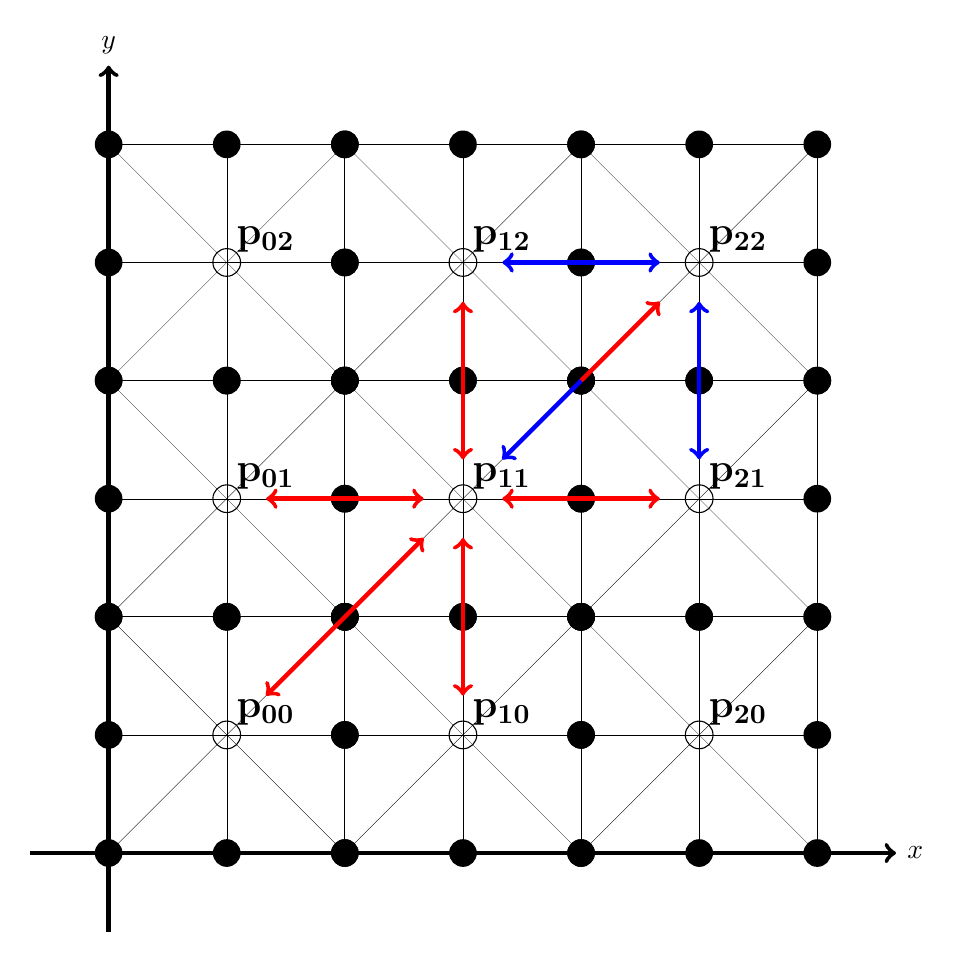
\begin{tikzpicture}

    % Draw the x and y axes
    \draw[->,ultra thick] (-1,0) -- (10,0) node[right] {$x$};
    \draw[->,ultra thick] (0,-1) -- (0,10) node[above] {$y$};

    % Draw process grid
    \foreach \i in {0,3,6,9} {
        \draw[thin] (\i,0) -- (\i,9);
        \draw[thin] (0,\i) -- (9,\i);
    }

    % Draw triangles and place dots on vertices
    \foreach \i in {0,3,6} {
        \foreach \j in {0,3,6} {
            % triangles
            \draw[ultra thin] (\i,\j) -- (\i+3,\j+3);
            \draw[ultra thin] (\i,\j+3) -- (\i+3,\j);
            \draw[ultra thin] (\i,\j+1.5) -- (\i+3,\j+1.5);
            \draw[ultra thin] (\i+1.5,\j) -- (\i+1.5,\j+3);

            % dots on vertices
            \fill[black] (\i,\j) circle (5pt);
            \fill[black] (\i+3,\j) circle (5pt);
            \fill[black] (\i,\j+3) circle (5pt);    
            \fill[black] (\i+3,\j+3) circle (5pt);
            \fill[black] (\i+1.5,\j) circle (5pt);
            \fill[black] (\i+1.5,\j+3) circle (5pt);
            \fill[black] (\i,\j+1.5) circle (5pt);
            \fill[black] (\i+3,\j+1.5) circle (5pt);
        }
    }

    % Add process labels
    \foreach \i in {0,1,2} {
        \foreach \j in {0,1,2} {
            \node at (3*\i+1.5,3*\j+1.5) [above right] {\Large $\mathbf{p_{\i\j}}$};
            \draw (3*\i+1.5,3*\j+1.5) circle (5pt);
        }
    }

    % Show neighbouring processes of p11
    \draw[->,red,ultra thick] (6,6) -- (7,7);
    \draw[<->,red,ultra thick] (2,2) -- (4,4);
    \draw[<->,red,ultra thick] (2,4.5) -- (4,4.5);
    \draw[<->,red,ultra thick] (5,4.5) -- (7,4.5);
    \draw[<->,red,ultra thick] (4.5,2) -- (4.5,4);
    \draw[<->,red,ultra thick] (4.5,5) -- (4.5,7);

    % Show neithering processes of p22
    \draw[<->,blue,ultra thick] (7.5,7) -- (7.5,5);
    \draw[<->,blue,ultra thick] (5,7.5) -- (7,7.5);
    \draw[<-,blue,ultra thick] (5,5) -- (6,6);



\end{tikzpicture}
